\section{Implantation de l'algorithme de formation d'image}
\label{sec:proj_backprojection}

\subsection{Choix de l'algorithme de formation d'images}\label{subsec:choix_algo_image}
Pour réaliser la formation d'images, plusieurs algorithmes peuvent être considérés. Or, notre porteur est destiné à être un drone relativement léger et donc sujet à d'importants écarts de trajectoires (roulis, tangage, lacet). Le premier critère est donc l'absence d'hypothèse de trajectoire linéaire dans les algorithmes. Dans ce cas, seul l'algorithme de Backprojection respecte cette condition. Toutefois, pour nuancer ces propos, l'algorithme RMA permet une assez bonne correction de la trajectoire grâce à l'interpolation. Mais là encore, l'intégration de chaque contribution de chaque pixel dans l'algorithme de Backprojection le rend plus robuste aux erreurs de phase. 

Un autre argument en faveur du RMA pourrait être sa plus faible complexité : $O(N^2\log(N))$ contre $O(N^3)$ pour le Backprojection. Cependant, dans ce projet, le traitement des données est réalisé post-mission donc aucune contrainte d'embarqué n'est considérée. 

Pour ces différentes raisons, nous faisons le choix d'utiliser l'algorithme de Backprojection pour la formation de nos images SAR.

\subsection{Implantation de l'algorithme Backprojection}\label{subsec:implem_BP}

La première implantation a consisté en la mise en place de l'algorithme basique, nous verrons par la suite qu'il nécessitera des adaptations pour correspondre à notre simulateurs et aux données expérimentales. 

La première étape consiste à définir la taille de notre grille image et les instants d'échantillonnage sur l'axe temps lent. Les paramètres physiques liés à notre plateforme nous permettent d'obtenir une résolution azimutale de l'ordre de $5~cm$ et une résolution en distance de l'ordre de $80~cm$. Afin de pouvoir visualiser les lobes secondaires, nous avons fait le choix d'appliquer un sur-échantillonnage à notre grille, en la définissant à $2.5~cm$ en distance et en azimut.

Ensuite, il faut définir les positions auxquelles le signal a été émis. Cette étape est primordiale pour le bon fonctionnement de l'algorithme. En effet, Backprojection réalise une sommation cohérente de tous les échantillons pour chaque pixel. Une sommation cohérente dépend de la phase qui elle-même dépend de la distance parcourue par l'onde. On en déduit qu'une mauvaise définition des positions d'émissions du porteur résultera en l'incapacité de l'algorithme à reconstruire des images d'autant plus que Backprojection n'est plus en capacité de former une image une fois le seuil de $\frac{\lambda}{8}$ dépassé. Dans cette première version, les données utilisées sont synthétiques, la position de départ est parfaitement connue, la vitesse de déplacement est exacte et la PRF aussi. Ainsi, il est aisé de déduire la distance entre deux émissions et donc le vecteur des positions du porteur grâce à l'expression suivante :
\begin{equation}
    Pos_{radar}(n) = n \cdot \left(\frac{v}{PRF}\right) \quad \text{pour } n \in \{0, 1, \dots, N_{pulse}-1\}.
\end{equation}
Les paramètres de base sont maintenant calculés ou définis, il faut passer à la réalisation de la boucle de rétroprojection en itérant sur chaque pixel de l'image finale. 

On commence par calculer la distance théorique du radar par rapport au pixel considéré, puis on en déduit l'ouverture synthétique théorique pour ce pixel précis. Cette ouverture varie avec la distance selon l'expression 
\begin{equation}
    L_{synth} = \frac{\lambda\cdot R}{2\cdot\delta_{az}}.
\end{equation}
Intuitivement, il faut penser à une lampe torche. En éclairant un mur à $2~m$ et à $10~m$ avec la même lampe, un point donné sur chacun des murs sera éclairé plus longtemps lorsque le mur se trouve à $10~m$ que lorsqu'il est présent à $2~m$. Ainsi, la quantité de contribution à la reconstruction de ce pixel est plus importante ce qui nous permet de maintenir une résolution azimutale constante sur toute la distance. Une fois l'ouverture synthétique calculée, il nous est possible de déterminer le nombre de points de l'axe azimut qui contribueront à la formation de ce pixel. 
Cependant, cette logique simpliste omet l'existence de cible avec un faible rayonnement. En effet, si une cible réfléchissante se trouve à proximité d'une cible moins réfléchissante, les lobes secondaires de la première vont submerger la réponse de la deuxième. Pour réduire cet effet, on utilise des fenêtres d'apodisation qui permettent de réduire l'impact des lobes secondaires au prix d'un élargissement du lobe principal.

Ensuite, il est nécessaire de définir la position du radar la plus proche de la cible pour en déduire l'intervalle des impulsions contribuant à la formation du pixel. Pour cela, on cherche le minimum de la valeur absolue de la différence entre la position du radar et celle du pixel en azimut. Puis, on détermine les bornes de notre intervalle en utilisant le nombre d'impulsions qui contribuent au pixel qui a été déterminé précédemment. Ce fonctionnement permet de simuler le passage du porteur face à la cible avec la phase d'approche et d'éloignement.

Une fois ces étapes réalisées, il ne reste plus que le cœur de l'algorithme, à savoir la sommation cohérente sur l'intervalle prédéfini. 

On commence par calculer la distance entre la position du radar à l'instant considéré et le pixel à reconstruire. Multipliée par deux, cette dernière correspond au chemin aller-retour réalisé par l'onde. On en déduit ensuite un temps de propagation qui sera utilisé pour retrouver l'index d'échantillon en temps rapide. L'interpolation utilisée est celle du plus proche voisin. Elle a été choisie pour sa rapidité d'exécution puisque cette implémentation a pour unique objectif de valider la formation d'image sur données synthétiques. Une fois les paramètres calculés, nous allons compenser la phase induite par la distance parcourue par l'onde afin de pouvoir additionner la contribution de cet échantillon au pixel considéré. Pour retirer la phase, nous multiplions le signal par l'exponentielle complexe $\exp(j2\pi f_c t_d)$ avec $f_c$ la fréquence d'émission et $t_d$ la durée de propagation de l'onde. On remarque par ailleurs l'impact d'une erreur de trajectoire sur la reconstruction de l'image puisque la compensation de phase se fait en fonction de la trajectoire supposée. 

Cette implémentation fonctionne avec un simulateur qui fournit l'intensité de l'écho perçu par la carte. Or, notre carte utilise une forme d'onde modulée continue, FMCW triangulaire. Ainsi, utiliser l'écho n'est pas possible puisque cela nécessiterait une fréquence d'échantillonnage (au moins 2x la bande de modulation). De plus, utiliser une telle méthode dans notre cas n'est pas pertinent et très coûteux. A la place, nous utiliserons la fréquence de battement issue de la carte. Il faut donc adapter l'implémentation de l'algorithme pour que cette dernière soit pertinente.

\subsection{Adaptation à l'architecture FMCW triangulaire et multi-canaux}\label{subsec:adapt_bp}

Afin de traiter les données réelles issues du capteur K-MC4, l'algorithme de rétroprojection a dû être profondément remanié pour s'adapter à une architecture FMCW triangulaire et multi-canaux. Contrairement au modèle précédent qui simulait l'émission d'impulsions courtes et mesurait un temps de vol direct, notre système émet un signal continu dont la fréquence varie linéairement. À la réception, le signal réfléchi est mélangé avec le signal émis instantanément, ce qui produit un signal dont la fréquence de battement est directement proportionnelle à la distance aller-retour de la cible. Cette spécificité matérielle rend la lecture temporelle directe obsolète.  L'algorithme intègre désormais une étape de pré-traitement systématique : une Transformée de Fourier Rapide est appliquée sur l'axe du temps rapide pour convertir les signaux bruts en spectres de fréquences.

La mécanique de la rétroprojection s'en trouve ainsi modifiée. La boucle n'itère plus pour extraire un indice temporel, mais convertit la distance géométrique bistatique (émetteur-cible-récepteur) en une fréquence de battement théorique cible. Cette fréquence permet de calculer l'indice précis dans le spectre pré-calculé. Étant donné que cet indice est rarement entier, l'interpolation au plus proche voisin a été remplacée par une interpolation linéaire, indispensable pour garantir la précision de la phase lue dans le spectre. Enfin, l'approche pixel par pixel pour définir l'ouverture synthétique a été simplifiée au profit d'une opération matricielle globale. Le fenêtrage d'azimut est désormais appliqué en amont sur l'ensemble de la trajectoire, et la contribution de chaque impulsion est projetée simultanément sur l'intégralité de la grille spatiale, optimisant ainsi les temps de calcul tout en intégrant la dimension tridimensionnelle de la trajectoire du porteur.

\subsection{Résultats}

Maintenant l'algorithme implémenté et adapté à notre simulateur, nous pouvons valider la formation d'image avec différentes configurations. La Figure \ref{fig:img_3bp} présente trois images reconstruites pour une cible ponctuelle située à $20~m$ du radar, générées avec une bande de fréquence de $250~MHz$.

La première image (à gauche) illustre le cas idéal sans perturbation : l'énergie est parfaitement focalisée. La deuxième image (au centre) introduit uniquement des erreurs d'attitude du porteur. On observe une dégradation nette de la focalisation, caractérisée par une élévation importante des lobes secondaires en azimut, symptôme direct des erreurs de phase lors de la sommation cohérente. Enfin, la troisième image (à droite) combine ces erreurs d'attitude avec l'ajout de clutter, ce qui masque les lobes secondaires et détériore fortement le contraste global de la scène.

\begin{figure}[hbt!]
    \centering
    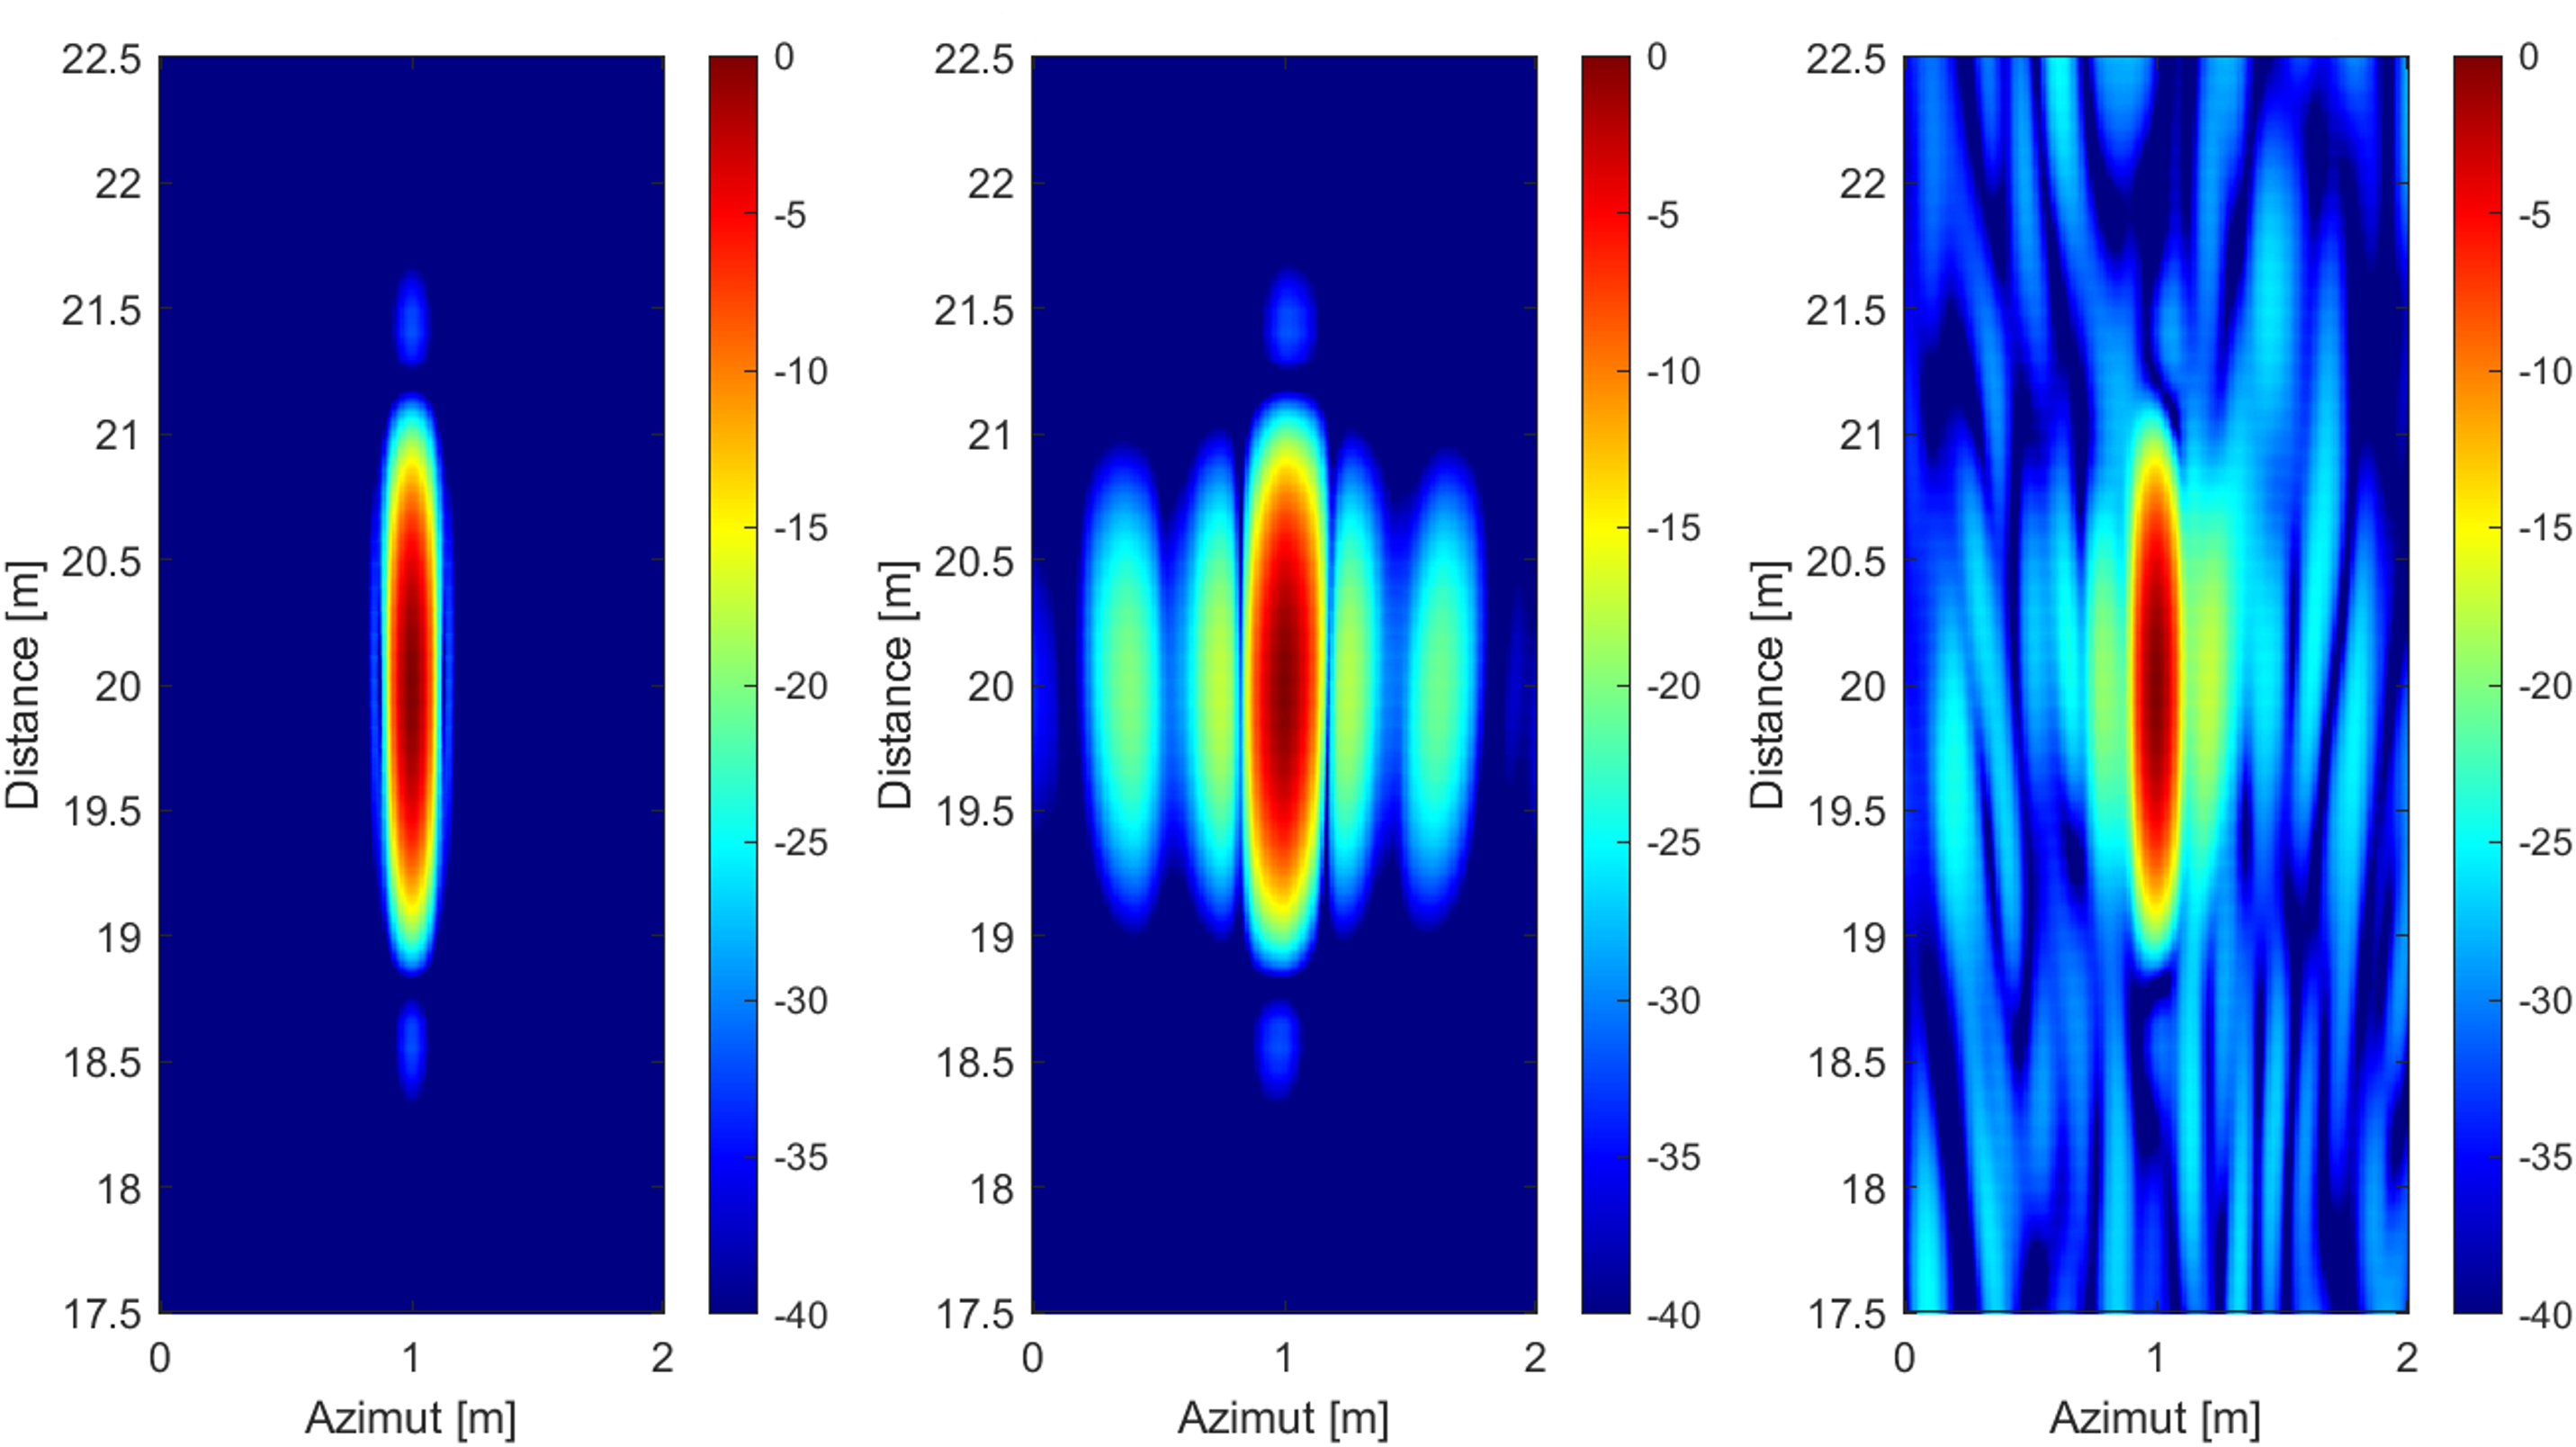
\includegraphics[width=0.9\linewidth]{src/rapport_complet/img/3bp.png}
    \caption{Images formées par l'algorithme de Backprojection}
    \label{fig:img_3bp}
\end{figure}

Ces résultats valident le bon fonctionnement de notre implémentation de l'algorithme Backprojection, tout en mettant en évidence sa forte sensibilité aux incertitudes de trajectoire. Il est donc indispensable de s'intéresser à la correction de ces erreurs de phase, ce qui fera l'objet de la partie suivante.
